\documentclass[conference]{IEEEtran}
\IEEEoverridecommandlockouts
\usepackage{fontspec}
% TeX Gyre: free Times, Helvetica and Courier designs, by file name for Tectonic.
\setmainfont{texgyretermes}[Extension=.otf, UprightFont=*-regular, BoldFont=*-bold, ItalicFont=*-italic, BoldItalicFont=*-bolditalic]
\setsansfont{texgyreheros}[Extension=.otf, UprightFont=*-regular, BoldFont=*-bold, ItalicFont=*-italic, BoldItalicFont=*-bolditalic]
\setmonofont{texgyrecursor}[Extension=.otf, UprightFont=*-regular, BoldFont=*-bold, ItalicFont=*-italic, BoldItalicFont=*-bolditalic, Scale=0.95]
\usepackage{amsmath}
\usepackage{booktabs}
\usepackage{graphicx}
\usepackage{xcolor}
\usepackage{tikz}
\usetikzlibrary{arrows.meta,positioning,fit,calc}
\usepackage[hidelinks]{hyperref}
\usepackage{url}
\usepackage{cite}

\definecolor{ink}{HTML}{15201A}
\definecolor{brand}{HTML}{0B6B45}
\definecolor{lcdbg}{HTML}{C7DAA9}
\definecolor{accent}{HTML}{B5501B}

% A keypad-phone screen, as the user sees it.
\newcommand{\lcd}[2]{%
  \begin{tikzpicture}
    \node[draw=ink!60, fill=lcdbg, rounded corners=2pt, inner sep=3pt, text width=#1, align=left,
          font=\ttfamily\fontsize{6.4}{7.6}\selectfont] {#2};
  \end{tikzpicture}}

\begin{document}

\title{Kalangu: AI Agents for Every Phone\\over USSD and SMS\\[4pt]
{\Large A Municipal Case Study in Ndi\'edieng, Senegal}}

\author{
\IEEEauthorblockN{Author Name}
\IEEEauthorblockA{\textit{Affiliation}\\
\textit{City, Country}\\
email@example.org}
\and
\IEEEauthorblockN{Author Name}
\IEEEauthorblockA{\textit{Affiliation}\\
\textit{City, Country}\\
email@example.org}
}

\maketitle

\begin{abstract}
Conversational AI is being built almost exclusively for smartphones and the
web, while a large part of the population in many African regions reaches
digital services through Unstructured Supplementary Service Data (USSD) codes
and SMS on basic phones, often without mobile data. Putting a language model
behind a USSD code is not a matter of connecting an API: USSD sessions expect
an application reply within about ten seconds, screens hold around 160
characters, and a single accented letter can cut an SMS's capacity from 160
to 70 characters. We present Kalangu, an open-source TypeScript toolkit that
reconciles these constraints through three ideas: \emph{typed turns} rendered
per channel, an \emph{encoding-aware budgeter} that never truncates, and
\emph{deferral}, which ends a USSD session gracefully when a model misses its
deadline and delivers the answer by SMS. We describe its design and a
prototype built with it for the commune of Ndi\'edieng (Kaolack, Senegal),
where village chiefs report broken boreholes, births and deaths by USSD, SMS
or voice, and the town hall queries its records through a voice assistant
that shows the data behind each answer and can answer in Wolof. Measured on
the built packages, fixed menus answer in under 1\,ms at the 95th percentile,
deferral closes the screen at the deadline and delivers the answer by SMS as
soon as the model finishes, all 41 screens of the prototype's menu tree fit in
160 characters, and a third of the messages in our Wolof and Hausa drafts
would be billed as Unicode SMS. We discuss what remains unverified, notably
behaviour on real operator networks.
\end{abstract}

\begin{IEEEkeywords}
USSD, SMS, feature phones, conversational agents, large language models, ICT4D, Senegal, Wolof
\end{IEEEkeywords}

% ---------------------------------------------------------------------------
\section{Introduction}

Over the last few years, everyday communication has moved quickly towards AI:
people ask chat assistants, talk to voice agents, and expect services to
answer at once. Almost all of this assumes a smartphone, an app and a data
connection. In many rural areas that assumption fails. What people do have
is a phone that can dial a code such as \texttt{*123\#} and send SMS, the two
channels through which services such as mobile money reached them in the
first place.

These channels are hard to build for. USSD is session-based and synchronous:
the network forwards each keypress to the application and waits, typically no
more than ten seconds, for the next screen~\cite{atdocs,athelp}. Screens are
small (160 characters on several operators), the operator paginates
over-long screens itself with reserved codes, and many characters cannot be
displayed. SMS is asynchronous but has its own trap: the GSM 7-bit alphabet
holds 160 characters per message, while one character outside it switches the
whole message to UCS-2 and 70 characters~\cite{3gpp23038}. Language models,
meanwhile, take seconds to answer and are verbose.

This paper makes four contributions:
\begin{enumerate}
  \item A design that reconciles language models with USSD and SMS: typed
  turns, an encoding-aware budgeter, and deadline-based deferral to SMS
  (Section~\ref{sec:design}).
  \item An open-source implementation, Kalangu, published as four packages
  with a terminal and scriptable phone simulator~\cite{kalanguRepo}.
  \item A case study: a working prototype for a Senegalese commune, including
  a read-only data assistant answering in French or Wolof
  (Section~\ref{sec:case}).
  \item Measurements of latency, deferral, encoding cost per language and
  screen budget on the built code (Section~\ref{sec:eval}), and a frank list
  of what is still unverified (Section~\ref{sec:limits}).
\end{enumerate}

% ---------------------------------------------------------------------------
\section{Background}
\label{sec:background}

\subsection{USSD}
USSD~\cite{3gpp22090} is reached by dialling a service code. Through the
Africa's Talking gateway used in this work, each request is an HTTP POST
carrying the session identifier, the phone number and a \texttt{text} field
that accumulates every input so far, joined by \texttt{*}; the application
answers with a body starting \texttt{CON} (continue) or \texttt{END}
(terminate)~\cite{atdocs,atnode}. The gateway documents an expected
application response time of at most 10\,s; Kenyan operators publish total
session lengths of 180\,s and screen limits of 160 (Safaricom) and 184
characters (Airtel), and paginate long screens themselves with reserved codes
\texttt{98} (more) and \texttt{00} (back)~\cite{athelp}. Menus must avoid
characters that handsets cannot render.

\subsection{SMS encoding}
An SMS segment carries 160 characters in the GSM 7-bit default alphabet (153
when concatenated), and characters from its extension table count
twice~\cite{3gpp23038}. Any character outside the alphabet forces UCS-2 for
the whole message: 70 characters, or 67 per concatenated segment. French
\textit{\'e}, \textit{\`e} and \textit{\`a} are in the GSM alphabet, but
\textit{\c{c}} and \textit{\^e} are not; neither are Wolof \textit{\"e} and
\textit{\ng}, nor the hooked (implosive) letters of Hausa. The cost of a
message is therefore a property of its language, which matters for agents
whose replies are generated rather than written in advance.

% ---------------------------------------------------------------------------
\section{Related Work}
\label{sec:related}

A survey of the npm registry in November 2026~\cite{kalanguRepo} found two
kinds of tools. Gateway SDKs such as the official Africa's Talking
SDK~\cite{atnode} wrap the HTTP API and leave session logic to the developer.
Menu builders such as \texttt{ussd-builder}~\cite{ussdbuilder},
\texttt{ussd-state-builder}~\cite{ussdstate} and \texttt{ananse}~\cite{ananse}
compose state machines of USSD menus, some with session stores, validation,
pagination and simulators. The closest prior art,
\texttt{@omoyolab/ussdkit}~\cite{ussdkit}, offers declarative screens, gateway
adapters, a terminal simulator and screen-room warnings. None of these
integrate a language model, defer slow answers to SMS within the gateway's
bound, or budget SMS by encoding; Kalangu's difference lies on that agent side
rather than in menus or sessions. Multi-channel chat frameworks follow the
same pattern: the Chat SDK adapter directory~\cite{chatsdk} lists adapters for
messaging platforms and SMS providers but none for USSD.

% ---------------------------------------------------------------------------
\section{Design}
\label{sec:design}

\begin{figure*}[t]
\centering
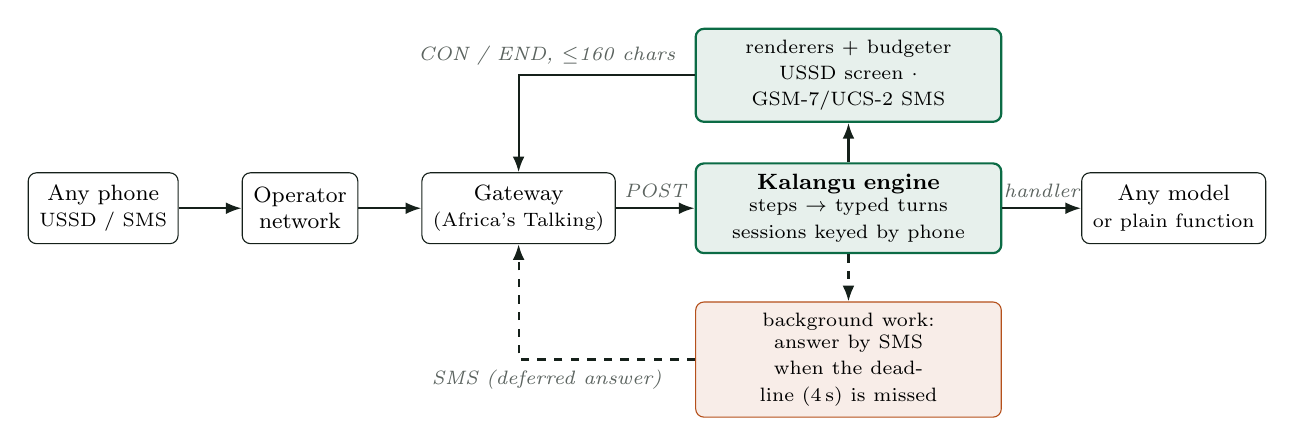
\begin{tikzpicture}[
  box/.style={draw=ink, rounded corners=3pt, align=center, font=\footnotesize, minimum height=9mm, inner sep=4pt},
  core/.style={box, fill=brand!10, draw=brand, thick},
  arr/.style={-{Latex[length=2mm]}, thick, ink},
  note/.style={font=\scriptsize\itshape, text=ink!70}]
  \node[box] (phone) {Any phone\\\scriptsize USSD / SMS};
  \node[box, right=8mm of phone] (op) {Operator\\network};
  \node[box, right=8mm of op] (gw) {Gateway\\\scriptsize (Africa's Talking)};
  \node[core, right=10mm of gw, text width=36mm] (engine) {\textbf{Kalangu engine}\\\scriptsize steps $\rightarrow$ typed turns\\\scriptsize sessions keyed by phone};
  \node[core, above=5mm of engine, text width=36mm] (render) {\scriptsize renderers + budgeter\\\scriptsize USSD screen $\cdot$ GSM-7/UCS-2 SMS};
  \node[box, right=10mm of engine] (model) {Any model\\\scriptsize or plain function};
  \node[box, below=6mm of engine, text width=36mm, fill=accent!10, draw=accent] (bg) {\scriptsize background work: answer by SMS\\\scriptsize when the deadline (4\,s) is missed};
  \draw[arr] (phone) -- (op);
  \draw[arr] (op) -- (gw);
  \draw[arr] (gw) -- node[above, note]{POST} (engine);
  \draw[arr] (engine) -- (render);
  \draw[arr] (render.west) -| node[above, pos=0.42, note]{CON / END, $\le$160 chars} (gw.north);
  \draw[arr] (engine) -- node[above, note]{handler} (model);
  \draw[arr, dashed] (engine) -- (bg);
  \draw[arr, dashed] (bg.west) -| node[below, pos=0.42, note]{SMS (deferred answer)} (gw.south);
\end{tikzpicture}
\caption{Architecture. Handlers return typed turns; a renderer per channel and the budgeter turn them into screens or SMS that fit. A model turn that misses its deadline ends the USSD session with a notice, and its answer is sent by SMS from background work.}
\label{fig:arch}
\end{figure*}

Figure~\ref{fig:arch} shows the architecture. An agent is a tree of
\emph{steps}: \texttt{menu}/\texttt{choose} (numbered options), \texttt{ask}
(free text or a number), \texttt{confirm} (yes/no), \texttt{say} (a final
message) and, experimentally, \texttt{pay}. Handlers receive the input and a
context holding the session, the locale and the model, and return a string, a
next step, or nothing. The whole agent is exposed as a standard
\texttt{Request}\,$\rightarrow$\,\texttt{Response} handler, so it runs on
Node.js, serverless platforms or in a browser.

\subsection{Typed turns}
Agents never write text directly to a phone. Each step produces a typed turn
(\texttt{say}, \texttt{choose}, \texttt{ask}, \texttt{confirm}), and a
renderer per channel converts it: a numbered menu on USSD, a numbered reply
list on SMS. Typed answers are matched to options regardless of accents,
case, spacing and apostrophe style, because USSD strips accents from labels
while users may type them.

\subsection{An encoding-aware budgeter that never truncates}
For USSD, text is restricted to a safe character set: accents are removed
(\textit{d\'eclarer} $\rightarrow$ \textit{declarer}), letters used in West
African orthographies are transliterated (\textit{\ng} $\rightarrow$
\textit{ng}), and anything else is removed and reported. Screens are laid out
under a configurable limit (160 by default) so that operator
auto-pagination never triggers; options are numbered around the reserved
codes, and long text is paged behind a \texttt{98} option that the agent
controls. For SMS, the budgeter counts GSM-7 septets (extension characters
twice) or UTF-16 units, splits at segment boundaries, reports which characters
forced UCS-2, and refuses (rather than truncates) a message beyond a segment
cap, four by default.

\subsection{Deferral}
Model-backed steps run under a deadline, 4\,s by default; the library warns
above 8\,s and refuses more than 10\,s, the gateway's bound. If the handler
answers in time, the answer is rendered on the screen. Otherwise the session
ends with a notice that an SMS is coming, the handler keeps running as
background work, and its answer is delivered by SMS when ready. Fixed menus
never call the model. On serverless platforms that freeze the process after
the response, the background hook must be bound to the platform's
\texttt{waitUntil} or a queue.

\subsection{Sessions, languages and safety}
Sessions are keyed by phone number with compare-and-set saves, so a
double-tapped confirmation cannot run twice; a dropped session resumes on
redial within five minutes. A language menu on first contact remembers each
number's choice; English and French ship, and community locales are checked
by a command that verifies placeholders and USSD/SMS fit. Phone numbers are
masked in logs. Because USSD gateways do not sign callbacks, deployments rely
on a secret path or an address allowlist.

\subsection{Testing without a SIM}
\texttt{@kalangu/sim} provides a keypad phone in the terminal and a scriptable
phone for tests, wired to the same engine through simulated USSD and SMS
channels, so an agent can be developed and tested with no operator, account
or API key.

% ---------------------------------------------------------------------------
\section{Case Study: Ndi\'edieng}
\label{sec:case}

\begin{figure}[t]
\centering
\begin{tabular}{@{}c@{\hspace{3mm}}c@{}}
\lcd{38mm}{Mairie de Ndiedieng\\1. Signaler une panne\\2. Declarer une naissance\\3. Declarer un deces\\4. Suivre un signalement\\5. Ecrire un message} &
\lcd{38mm}{Urgence ?\\1. Urgent : service coupe\\2. Genant, marche encore\\3. Peut attendre\\~\\~} \\[1mm]
\scriptsize (a) Root menu & \scriptsize (b) Urgency \\[2mm]
\multicolumn{2}{c}{\lcd{80mm}{Signalement S-0001 enregistre : forage, Village 12, urgence haute. Un SMS vous dira quand il est traite.}} \\[1mm]
\multicolumn{2}{c}{\scriptsize (c) Confirmation}
\end{tabular}
\caption{Real screens of the prototype, captured from the simulator: (a) the root menu, 134 characters; (b) the urgency question after \emph{Water}\,$\rightarrow$\,\emph{Borehole}; (c) the confirmation. The budgeter removes accents for USSD.}
\label{fig:screens}
\end{figure}

Ndi\'edieng is a rural commune in the Kaolack region of Senegal. In
conversations around a local call for digital projects, the problem described
was simple: when a borehole stops or a health post loses power, the village
chief travels or calls informally to warn the town hall; nothing is recorded
or followed up, and the town hall decides without an overview. We built a
prototype with Kalangu~\cite{kalanguDemo}. Its data is generated and fictitious:
58 villages, 200 pieces of equipment and 499 territorial records.

\subsection{The village side}
A chief dials \texttt{*123\#} and reports a breakdown (type, equipment,
urgency), a birth or a death, follows up a report, or writes a message
(Fig.~\ref{fig:screens}). Each report receives a number. Free SMS and voice
messages are classified into category, equipment and urgency with a
confidence; under 0.6 the report goes to a ``to check'' queue where a person
decides. When the town hall takes a report on or resolves it, the chief
receives an SMS. Births and deaths are pre-declarations that alert the town
hall; the civil registration act follows the legal procedure.

\subsection{The town hall side}
A dashboard lists reports by status and urgency; staff can open, edit,
create and delete them, and equipment states follow their open reports. An
assistant answers questions such as ``which boreholes are broken?'' from the
commune's tables and always shows the query and the rows used. Without a
model it answers common questions with queries written in advance; with
Gemini~\cite{gemini}, the model writes one \texttt{SELECT}, which runs only if
a checker accepts it (a single read-only statement with no forbidden keyword)
and only on a read-only connection or a throwaway copy, and the model then
words the answer from the returned rows.

\subsection{Voice, Wolof, and running without a server}
The assistant is driven by voice. Because browsers' built-in recognition is
absent or silent in several of them and knows no Wolof~\cite{webspeech}, the
page records the question itself, stops at a pause judged against the room's
own noise, and sends a WAV file for transcription; the transcription reports
the question's language, and the written and spoken answers follow it, so a
question asked in Wolof is answered in Wolof. The model's key stays on the
server in a small function that accepts only fixed tasks (write a query, word
an answer, classify a message, transcribe, speak), with size limits, an
origin check and a per-visitor rate limit. On the public website, the whole
prototype, including SQLite compiled to WebAssembly~\cite{sqljs}, runs in the
visitor's browser and is kept in local storage; the same code runs on Node.js
behind the real gateway.

% ---------------------------------------------------------------------------
\section{Evaluation}
\label{sec:eval}

We measured the built packages on an Apple M3 Pro (11 cores, 18\,GB) with
Node.js 26.12, using the simulator and no network. The benchmark script and
its raw output are in the repository (\texttt{papers/kalangu/bench}).

\subsection{Fixed-menu latency}
We ran 500 complete USSD sessions through the full Ndi\'edieng agent, with
SQLite on disk: dial, then four keypresses to file a breakdown, which writes a
report. Table~\ref{tab:latency} shows that engine time is negligible against
the 10\,s bound: 0.63\,ms per request and 1.1\,ms per complete session at the
95th percentile. Network round trips, not the engine, dominate on real
deployments.

\begin{table}[t]
\centering
\caption{Fixed-menu latency through the Ndi\'edieng agent (ms)}
\label{tab:latency}
\begin{tabular}{@{}lrrrrr@{}}
\toprule
 & $n$ & p50 & p95 & p99 & max \\
\midrule
Per request & 2500 & 0.03 & 0.63 & 0.95 & 4.08 \\
Per session (5 requests) & 500 & 0.70 & 1.11 & 1.60 & 6.15 \\
\bottomrule
\end{tabular}
\end{table}

\subsection{Deferral}
An agent's model was made to take 6\,s against the default 4\,s deadline,
and 1.5\,s for comparison, three runs each. With the slow model, the USSD
screen returned after 4.00\,s (4001--4004\,ms) with the notice ``We are
working on your question. You will receive an SMS shortly'', and the answer
arrived by SMS at 6.00--6.01\,s, i.e.\ as soon as the model finished. With the
fast model, the answer was shown on the screen at 1.50\,s and no SMS was sent.
The user is never left facing a gateway timeout.

\subsection{Encoding cost by language}
We computed the SMS encoding of the 32 built-in messages (navigation,
confirmations, errors, deferral notices) in each locale
(Table~\ref{tab:encoding}). English never leaves GSM-7, and French does so for
3 messages because of \textit{\c{c}} and \textit{\^e}. In the machine-drafted
Wolof and Hausa locales, a third of the messages would be billed as Unicode
SMS: Wolof because of \textit{\"e}, Hausa because of its hooked letters;
Swahili, written in plain Latin letters, stays in GSM-7. These locales are
unreviewed drafts, so the figures describe their orthographies more than
their final wording; the point is that the same agent costs more to run in
some languages, and that the budgeter makes this visible before sending.

\begin{table}[t]
\centering
\caption{SMS encoding of the 32 built-in messages per locale}
\label{tab:encoding}
\begin{tabular}{@{}lrrl@{}}
\toprule
Locale & UCS-2 & Share & Characters forcing UCS-2 \\
\midrule
English (built in) & 0 & 0\% & -- \\
French (built in) & 3 & 9\% & \c{c} (2), \^e (1) \\
Wolof (draft) & 11 & 34\% & \"e (11) \\
Hausa (draft) & 12 & 38\% & hooked d (7), b (6), k (2) \\
Swahili (draft) & 0 & 0\% & -- \\
\bottomrule
\end{tabular}
\end{table}

\subsection{Screen budget}
Walking the prototype's whole menu tree (to depth four) visited 41 distinct
screens: none exceeded 160 characters; the longest, the root menu, has 134,
and the mean is 91.4. No screen would trigger operator pagination.

\subsection{Voice pipeline (indicative)}
With the prototype's serverless function running locally and a recorded
French question fed to the page's recorder, speech was detected after 0.8\,s, the recording stopped at
the pause, Gemini's transcription was exact (``Quels forages sont en panne
?''), and the spoken answer began about 4\,s after the answer text, once
answers were synthesised sentence by sentence. A Wolof question, spoken by
the model's own voice, was transcribed, answered correctly in Wolof, and
spoken. These are single observations on one connection, not a performance
study, and the free tier's speech quota was reached during testing.

\subsection{Tests}
The repository runs 587 automated tests on every change (504 across the four
packages, 83 across the two examples) and 47 on its build scripts, on Node.js
22 and 24, with a runtime smoke test on Node.js 20.

% ---------------------------------------------------------------------------
\section{Discussion and Limitations}
\label{sec:limits}

\textbf{No real operator yet.} All measurements use the simulator. Session
timeouts, screen limits, whether an operator intercepts \texttt{98}, and
whether a USSD session and an SMS to the same number work together
(on which deferral depends) must be verified on each operator; the published
figures we rely on are Kenyan. \textbf{No user study.} The prototype has not
yet been used by village chiefs; a field test with them is planned.
\textbf{Languages.} Wolof, Hausa and Swahili strings are machine drafts that
native speakers must review, and transcription and answers in Wolof were
tested only with model-generated speech. \textbf{Generated queries.} The
assistant's queries are constrained to one read-only statement and executed
where they cannot write, and every answer exposes its data, but a wrong yet
valid query can still produce a wrong answer, as we observed before adding
the exact stored values to the prompt. \textbf{Cost and dependence.} USSD
sessions and SMS are billed by operators; the voice features depend on a
commercial model API with quotas. The core flows (USSD, SMS, dashboard,
rule-based answers) work without any model.

% ---------------------------------------------------------------------------
\section{Conclusion}

Kalangu shows that an AI agent can be reached from any phone by treating the
channel's constraints (the deadline, the screen, the encoding) as first-class
design elements rather than afterthoughts. The Ndi\'edieng prototype turns
this into a service a commune could run: chiefs report in a few keypresses,
the town hall acts and replies by SMS, and staff ask questions aloud, in
French or Wolof, with the evidence shown. Next steps are field testing with
village chiefs, trials on operator networks, native-speaker review of the
Wolof and S\'er\`ere strings, and the payment and WhatsApp channels already
designed.

\section*{Availability}
Source code (MIT): \url{https://github.com/utachicodes/kalangu}. Live
prototype: \url{https://kalangu.utachi.website/ndiedieng/}. Benchmark and raw
results: \texttt{papers/kalangu/bench} in the repository.

\section*{Acknowledgment}
[Acknowledgments.]

\bibliographystyle{IEEEtran}
\bibliography{refs}

\end{document}
